\section{Image Classification - MNIST: CNN}
\label{sec:Image Classification - MNIST:CNN}

\subsection{Environment Setup}

The code starts by clearing all variables, closing all figures, and clearing the console. A parallel pool is started for parallel computation if it doesn't already exist.

\begin{lstlisting}[style=Matlab-editor]
clear all;
close all;
clc;
if isempty(gcp('nocreate'))
    parpool;
end
\end{lstlisting}

\subsection{Data Loading and Preprocessing}

The MNIST dataset is loaded into variables, reshaped, and normalized to have pixel values between \(0\) and \(1\).

\begin{lstlisting}[style=Matlab-editor]
data = load('mnist.mat');
trainImages = reshape(trainImages, [28, 28, 1, size(trainImages, 3)]);
trainImages = double(trainImages) / 255;
\end{lstlisting}

\subsection{CNN Architecture Definition}

The Convolutional Neural Network (CNN) architecture is defined. It comprises Convolution-BatchNorm-ReLU blocks, MaxPooling layers, a fully connected layer, a softmax layer, and a classification layer.

\begin{lstlisting}[style=Matlab-editor]
lgraph = layerGraph([ ... ]);
\end{lstlisting}

\subsection{Training Configuration}

Training options are defined, which include the choice of optimizer (Adam), learning rate, and number of epochs among other settings.

\begin{lstlisting}[style=Matlab-editor]
options = trainingOptions('adam', ...);
\end{lstlisting}

\subsection{Model Training and Evaluation}

The CNN model is trained, and its performance is evaluated on the test data to compute the accuracy.

\begin{lstlisting}[style=Matlab-editor]
[net, info] = trainNetwork(trainImages, categorical(trainLabels), lgraph, options);
pred = classify(net, testImages);
accuracy = sum(pred == categorical(testLabels)) / numel(testLabels);
\end{lstlisting}

\subsection{Metrics Calculation}

Precision, recall, and F1-score are calculated for each class based on the confusion matrix.

\begin{lstlisting}[style=Matlab-editor]
% Calculate precision, recall, and F1-score
\end{lstlisting}

\subsubsection{Network Design}

\begin{itemize}
    \item \textbf{Input Layer}: Accepts grayscale images of size \(28 \times 28 \times 1\).
    \item \textbf{Convolution Layers}: Two layers with \(3 \times 3\) filters. The first has 8 filters, and the second has 16.
    \item \textbf{Batch Normalization Layers}: Used for normalizing the activations.
    \item \textbf{ReLU Layers}: Used for introducing non-linearity.
    \item \textbf{Max-Pooling Layers}: Used for downsampling the feature maps.
    \item \textbf{Fully Connected Layer}: A dense layer with 10 output neurons for the 10 classes in MNIST.
    \item \textbf{Softmax and Classification Layers}: Used for multi-class classification.
\end{itemize}
\pagebreak
\section{Image Classification - MNIST: KNN}
\label{sec:Image Classification - MNIST:KNN}

\subsection{Environment Setup}
The initialization segment of the code sets up the MATLAB environment. By executing commands `close all;`, `clear all;`, and `clc;`, it ensures the workspace is clear from variables, closes all open figure windows, and cleans the Command Window. This is a standard practice to ensure that old data or figures do not interfere with new operations. Furthermore, a parallel pool is initiated to speed up certain computational tasks, especially when leveraging multi-core processors.
\begin{lstlisting}[style=Matlab-editor]
clear all;
close all;
clc;
if isempty(gcp('nocreate'))
    parpool;
end
\end{lstlisting}
\subsection{Data Loading and Preprocessing}
After setting up the environment, the code proceeds to load the MNIST dataset. The MNIST dataset is a collection of handwritten digits, commonly used in the field of machine learning and computer vision for training and testing algorithms related to image processing.

Subsequently, the data is separated into training and testing sets. Reshaping images into vectors is a common preprocessing step before feeding them into many machine learning algorithms.
\begin{lstlisting}[style=Matlab-editor]
data = load('mnist.mat');
training_set = data.training;
test_set = data.test;
train_Labels = gpuArray(training_set.labels);
test_Labels = gpuArray(test_set.labels);
\end{lstlisting}
To simplify the representation for the algorithms, each image is reshaped into a vector and the reshaped data is then transferred to GPU.

\begin{lstlisting}[style=Matlab-editor]
trainData = gpuArray(reshape(training_set.images, [], size(training_set.images, 3))');
testData = gpuArray(reshape(test_set.images, [], size(test_set.images, 3))');
\end{lstlisting}


\subsection{Principal Component Analysis (PCA)}

PCA is utilized to reduce data dimensionality. Here's a summary of its application to our dataset:

\subsubsection{PCA on Training Data}

Principal component vectors, representations, and variances are computed with:
\begin{lstlisting}[language=Matlab]
[coeff, score, latent] = pca(gather(trainData));
\end{lstlisting}

\subsubsection{Selecting Principal Components}

To retain \(95\%\) of the variance:
\begin{lstlisting}[language=Matlab]
explainedVariance = cumsum(latent) / sum(latent);
numComponents = find(explainedVariance > 0.95, 1);
\end{lstlisting}

\subsubsection{Data Projection}

Training data is mapped to the PCA space directly from the `score`. Test data is centered using the training mean and then projected:
\begin{lstlisting}[language=Matlab]
trainDataPCA = gpuArray(score(:, 1:numComponents));
meanTrain = mean(trainData, 1);
testDataPCA = gpuArray((gather(testData) - meanTrain)...
 * coeff(:, 1:numComponents));
\end{lstlisting}

These transformed datasets can be used for further tasks with reduced computational costs.




\subsection{Data Visualization}
Visualizing data is essential for understanding and interpreting results. In this code, two plots are constructed. The first plot shows the proportion of variance explained by each principal component, while the second illustrates the cumulative variance. These plots are valuable in comprehending the diminishing returns of including more components in the analysis.
\begin{figure}[h]
    \centering
    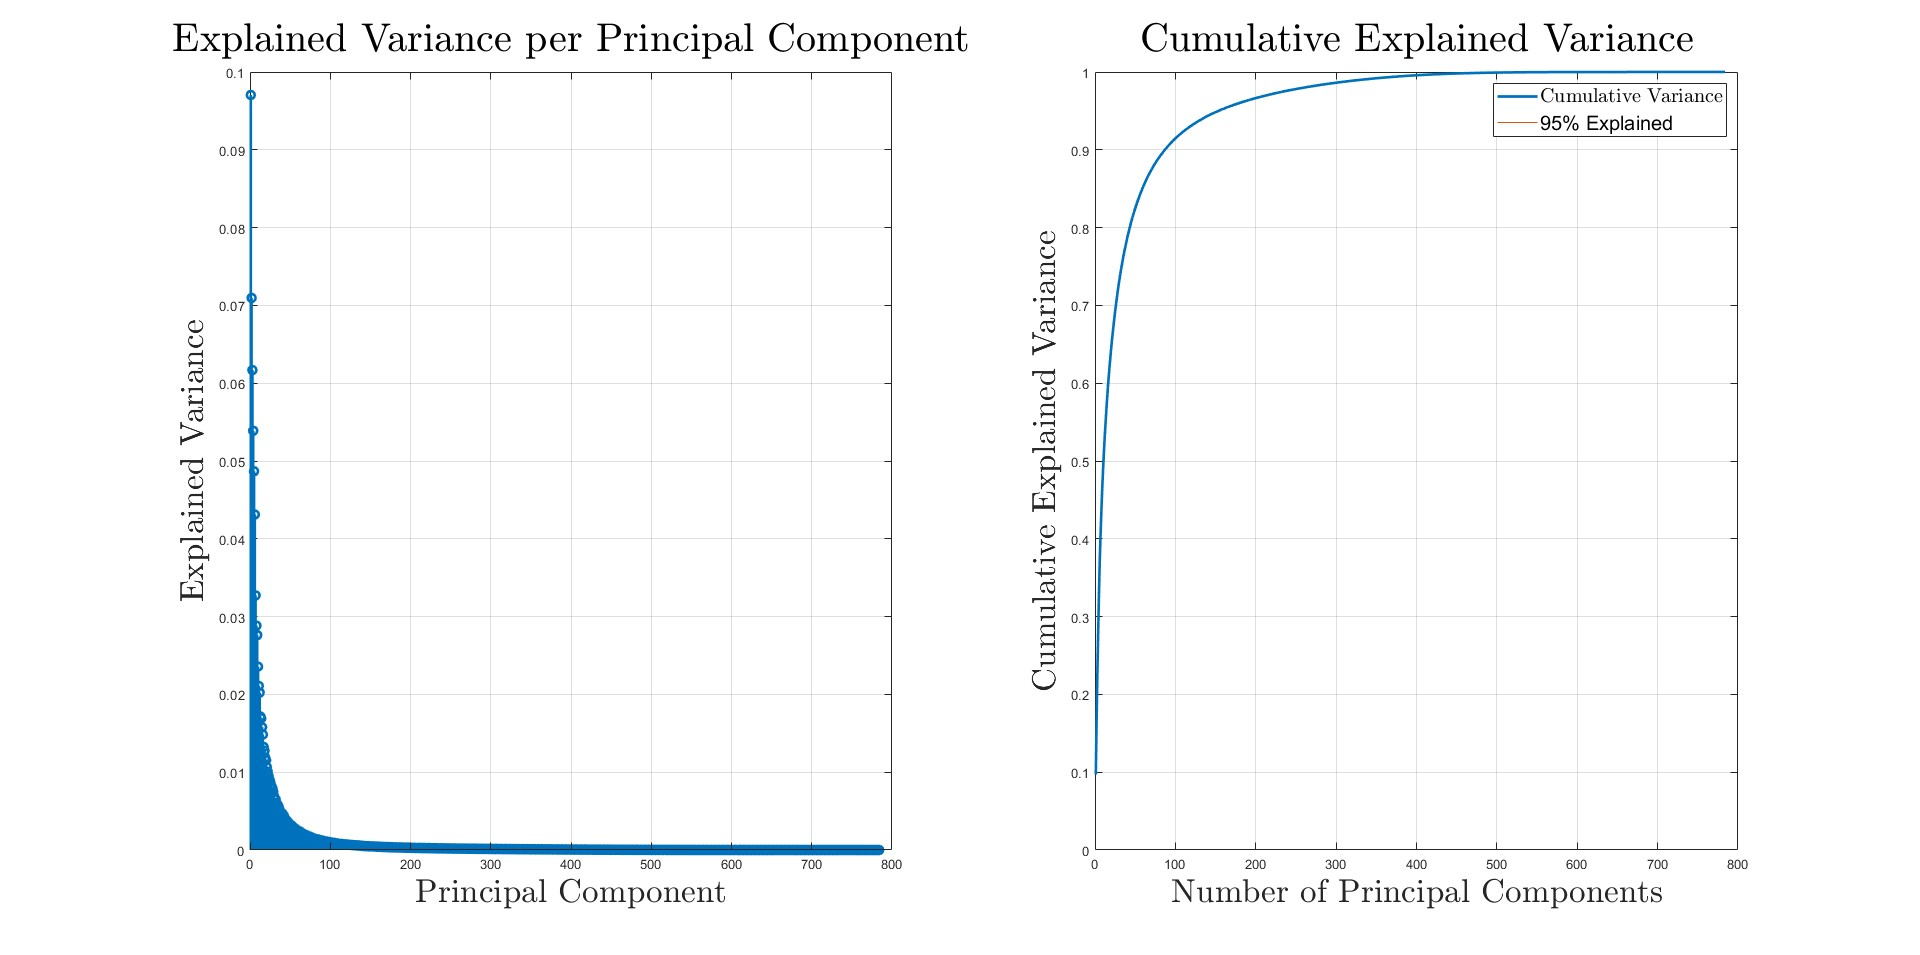
\includegraphics[width=1\textwidth]{PCA_KNN.jpg}
    \caption{Explained Variance Plot.}
    \label{fig:my_label} % optional, for referencing
\end{figure}
Two plots are generated for visualization:
\begin{itemize}
    \item The first plot illustrates the proportion of variance explained by each principal component.
    \item The second plot displays the cumulative variance explained by the principal components.
\end{itemize}
\subsection{k-Nearest Neighbors Classification}
The k-NN algorithm is a non-parametric method used for classification tasks. Here, the k-NN model is trained using PCA-transformed training data. The number of neighbors (`k`) is set to 5, with distance measured using correlation and weighted by the squared inverse. After training, predictions are made for the test set.

\subsection{Evaluation Metrics}
Performance evaluation is crucial to understanding how well the classifier works. The confusion matrix, a table layout of actual versus predicted classifications, is presented. From this matrix, various metrics such as precision, recall, and F1-score for each class are calculated. These metrics provide a more comprehensive view of the classifier's performance beyond just accuracy.

\subsection{Conclusions}
The provided code offers a comprehensive workflow for classifying the MNIST dataset using k-NN after dimensionality reduction with PCA. The inclusion of visualization tools and performance metrics ensures a robust understanding of the process and outcomes.


